% \documentclass{book}

\documentclass[12pt]{article}
\usepackage[pdfborder={0 0 0.5 [3 2]}]{hyperref}%
\usepackage[left=1in,right=1in,top=1in,bottom=1in]{geometry}%
\usepackage[shortalphabetic]{amsrefs}%
\usepackage{amsmath}
\usepackage{enumerate}
\usepackage{enumitem}
\usepackage{amssymb}                
\usepackage{amsmath}                
\usepackage{amsfonts}
\usepackage{amsthm}
\usepackage{bbm}
\usepackage[table,xcdraw]{xcolor}
\usepackage{tikz}
\usepackage{float}
\usepackage{booktabs}
\usepackage{svg}
\usepackage{mathtools}
\usepackage{cool}
\usepackage{url}
\usepackage{graphicx,epsfig}
\usepackage{makecell}
\usepackage{array}

\def\noi{\noindent}
\def\T{{\mathbb T}}
\def\R{{\mathbb R}}
\def\N{{\mathbb N}}
\def\C{{\mathbb C}}
\def\Z{{\mathbb Z}}
\def\P{{\mathbb P}}
\def\E{{\mathbb E}}
\def\Q{\mathbb{Q}}
\def\ind{{\mathbb I}}

\graphicspath{ {images11/} }

\begin{document}

\section*{25 March 2017}

\subsection*{Exponential Decay}
Let's look at the exponential decay rate of the various pulses and see if it's what we predict using the real part of the eigenvalue for the linearization about the 0-solution. For convenience, we can write the four nonzero eigenvalues of the linearization about the 0-solution as $\pm \mu \pm i \nu$. We expect $\mu$ to be the decay rate. Let's look at semilog plots for various values of $c$ and see if this is the case. Each plot has a best-fit line; the title contains the slope as well as the value of $\mu$.

\begin{figure}[H]
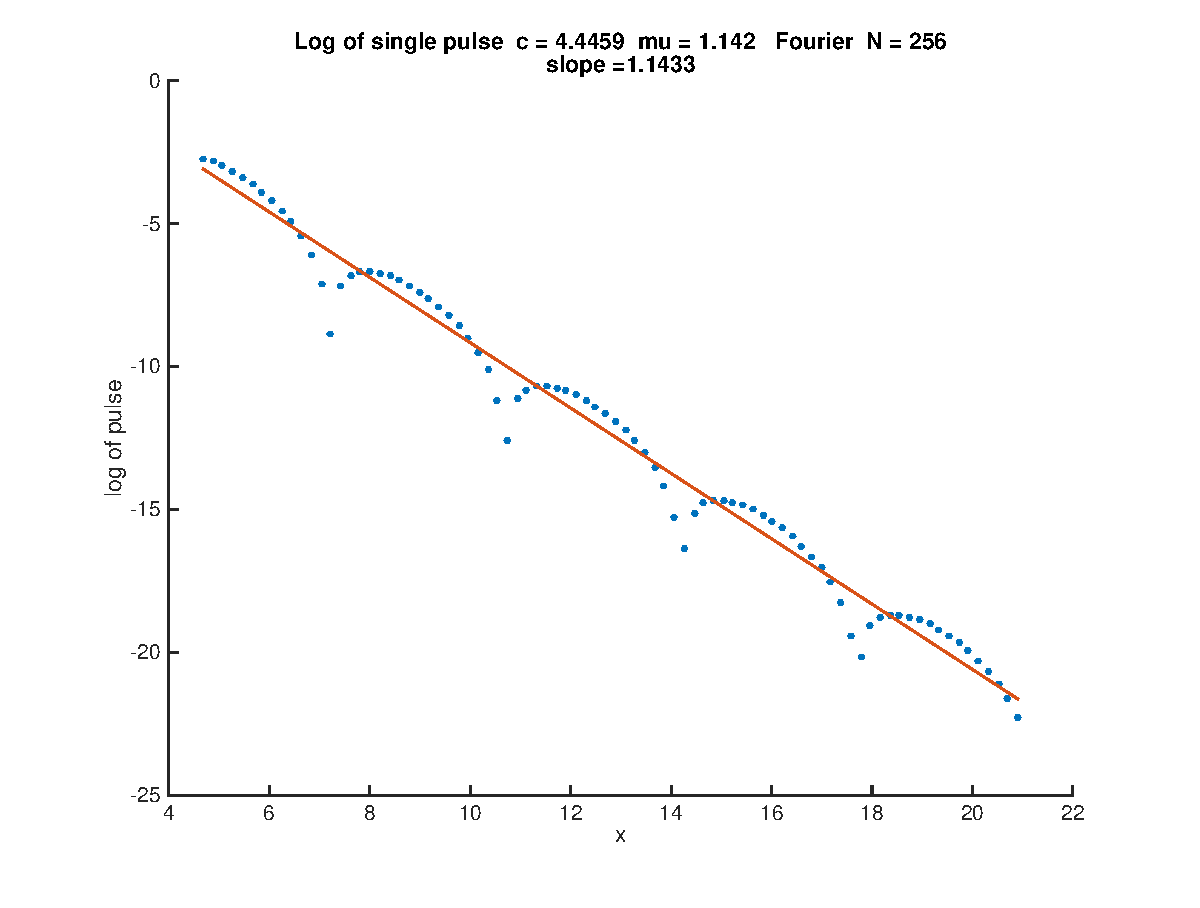
\includegraphics[width=8.5cm]{logsingle444.eps}
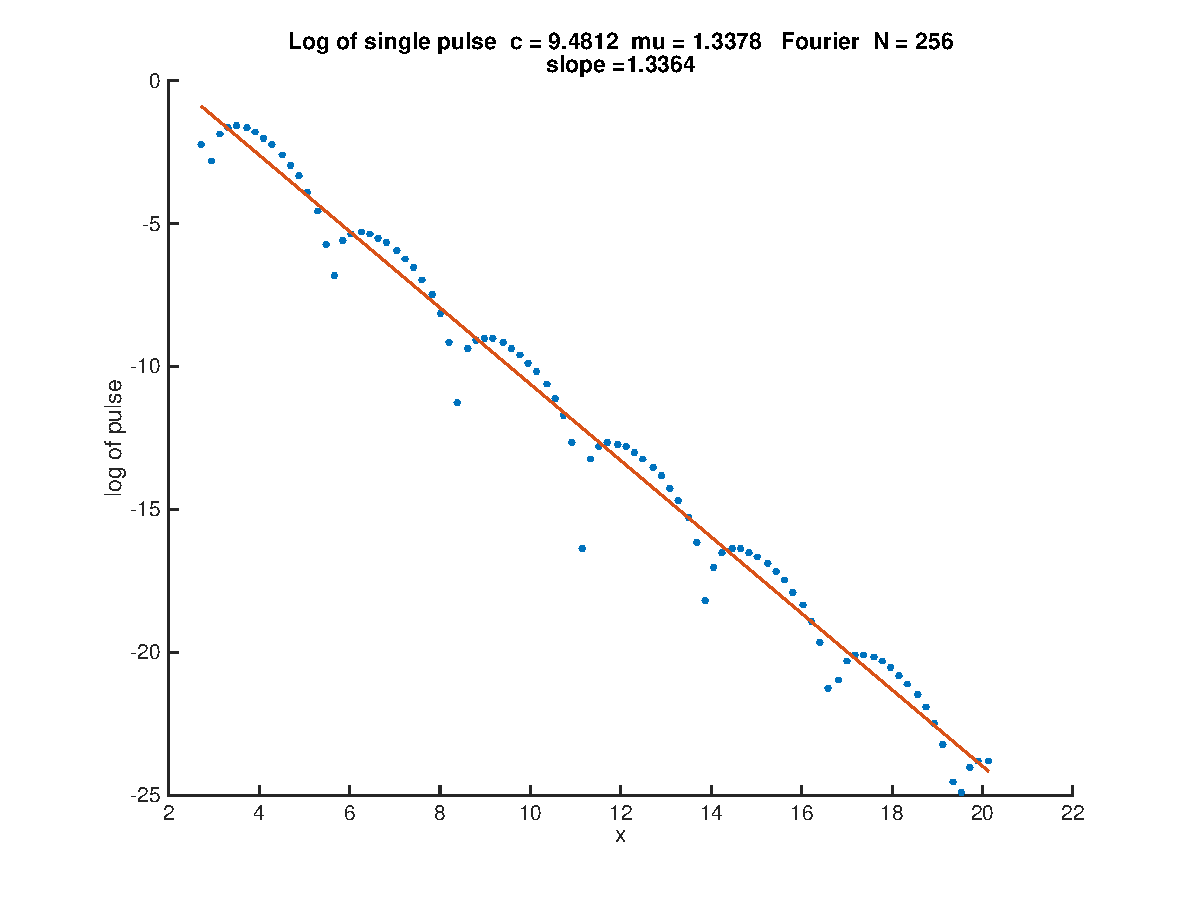
\includegraphics[width=8.5cm]{logsingle948.eps}
\end{figure}

\begin{figure}[H]
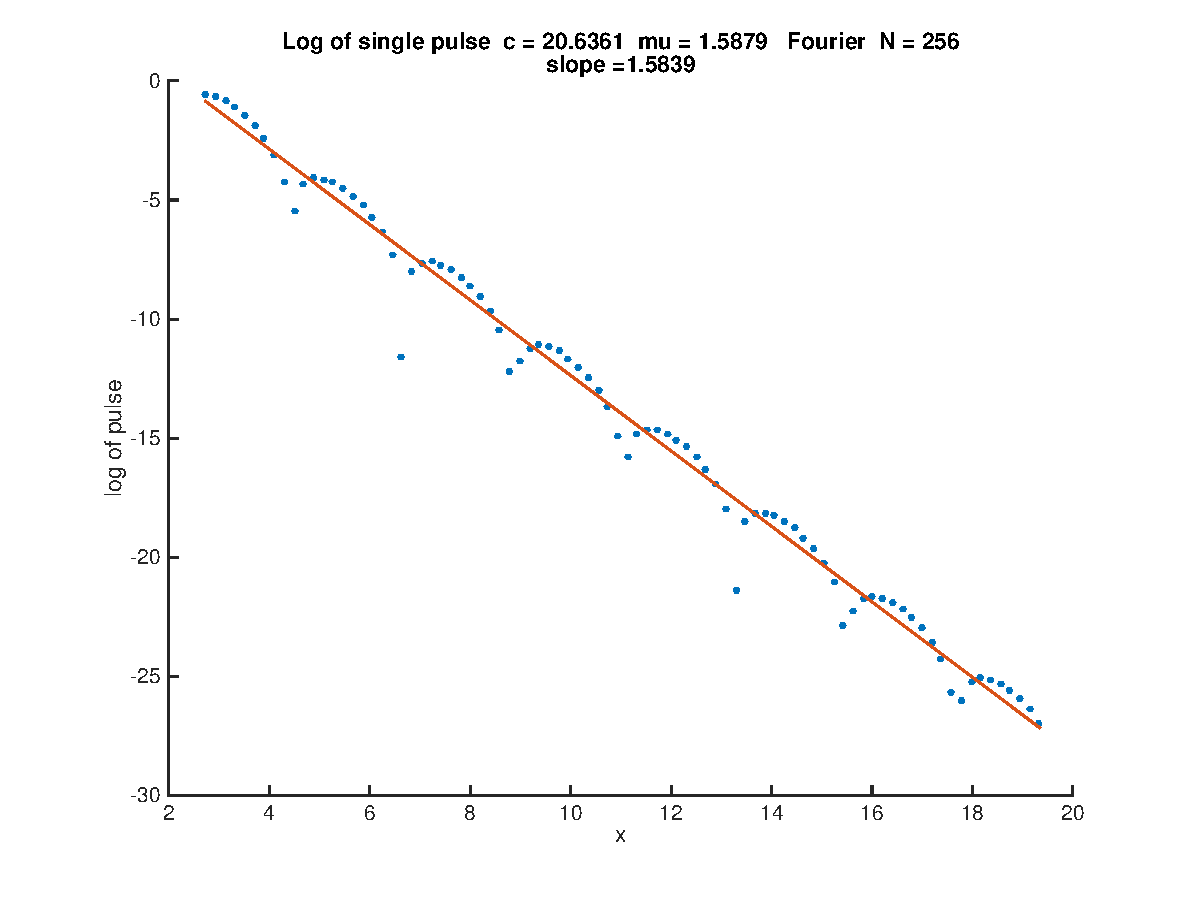
\includegraphics[width=8.5cm]{logsingle206.eps}
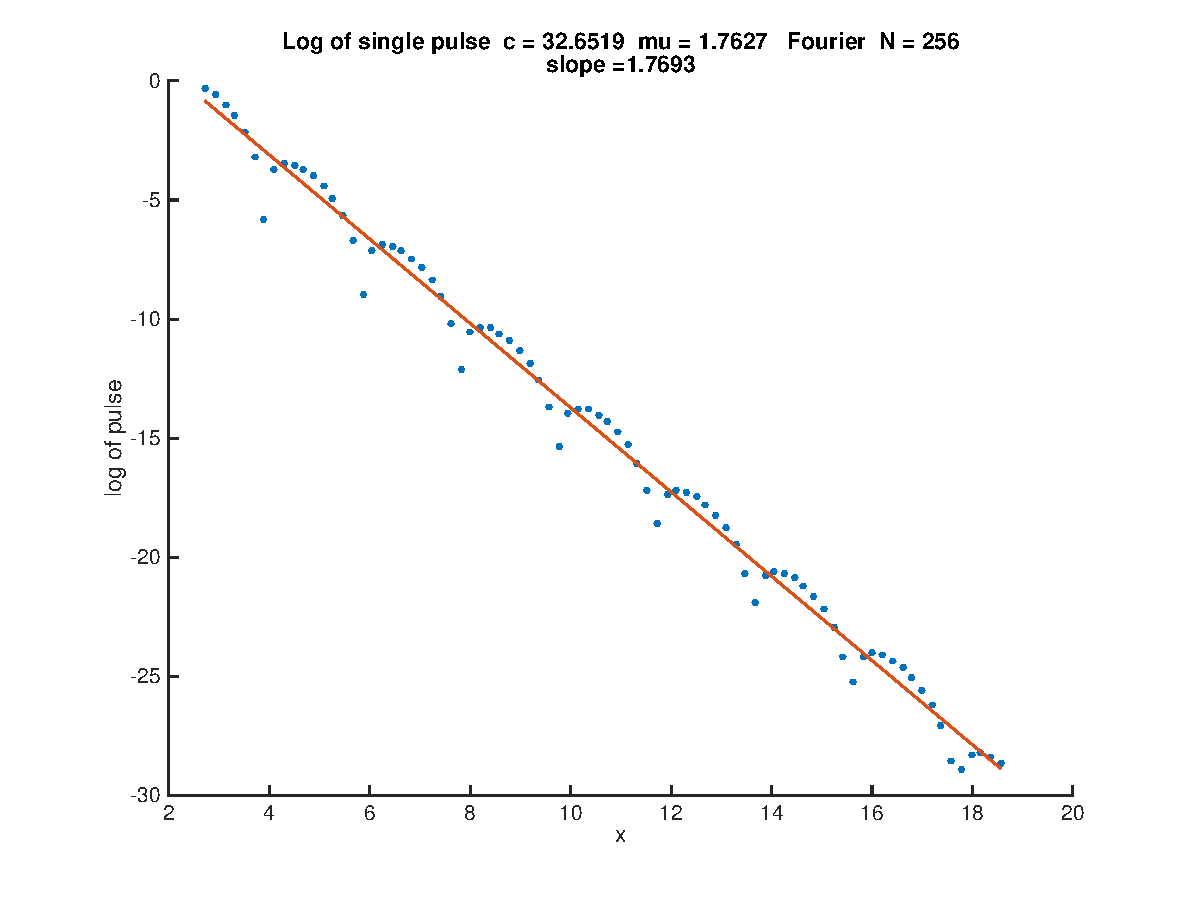
\includegraphics[width=8.5cm]{logsingle326.eps}
\end{figure}

The slopes match $\mu$ well in all cases, which is good. Unsurprisingly, this holds for our constructed double pulses as well (not shown).\\

Although it's nice that the above works, we are actually interested in the exponential decay rates of the eigenfunctions corresponding to the pure imaginary eigenvalues (the ones we get from even-numbered double pulses). What do we expect to get? If we take the spatial eigenvalues of the asymptotic matrix $A(\lambda)$ corresponding to the linearized eigenvalue problem, the real part of the negative eigenvalue with real part closest to 0 (slowest decay rate) should correspond to the decay rate of the eigenfunction. The eigenvalues of the asymptotic matrix are the roots of the characteristic polynomial $\lambda - c t + t^3 - t^5$. Let $\mu$ be the real part of the negative eigenvalue with real part closest to 0. Let's look at semilog plots of the eigenfunctions for four different values of $c$.

\begin{figure}[H]
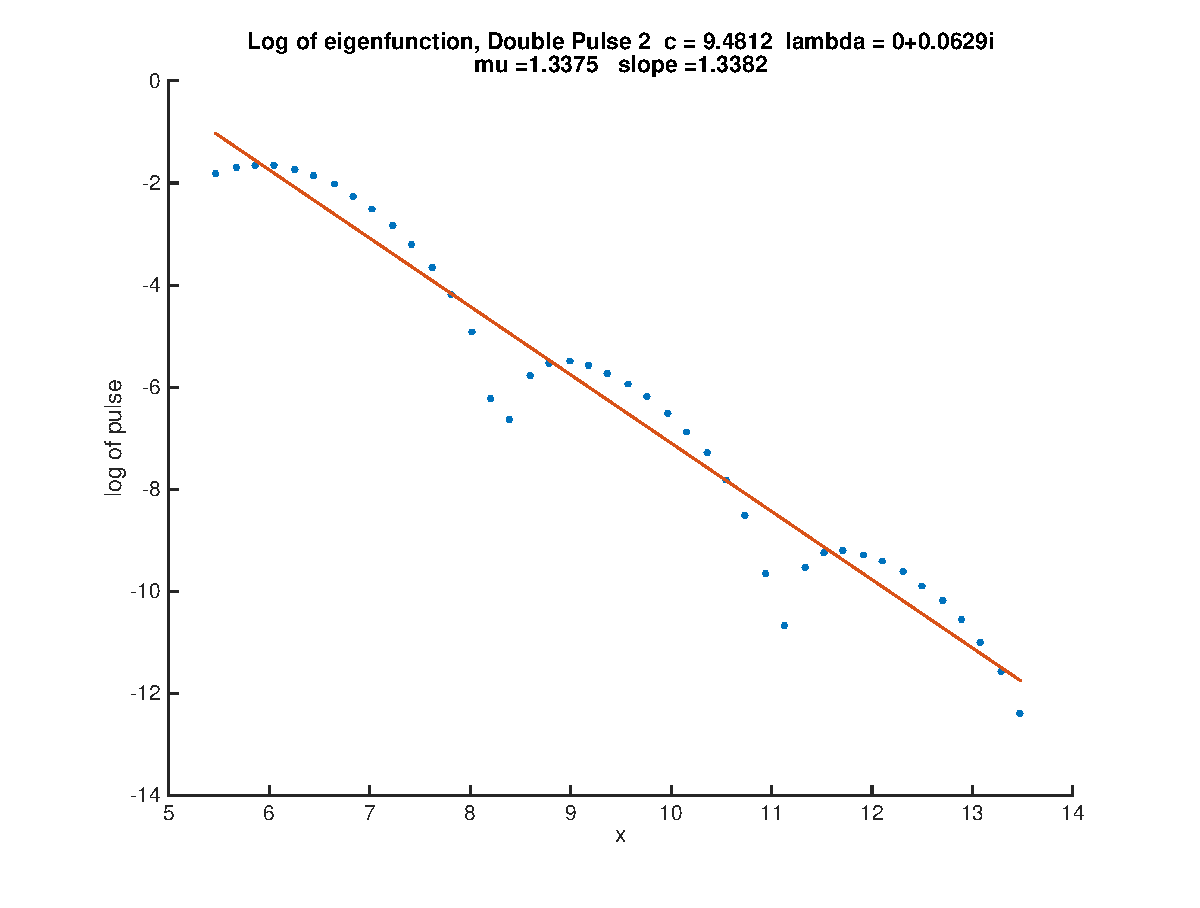
\includegraphics[width=8.5cm]{decay1.eps}
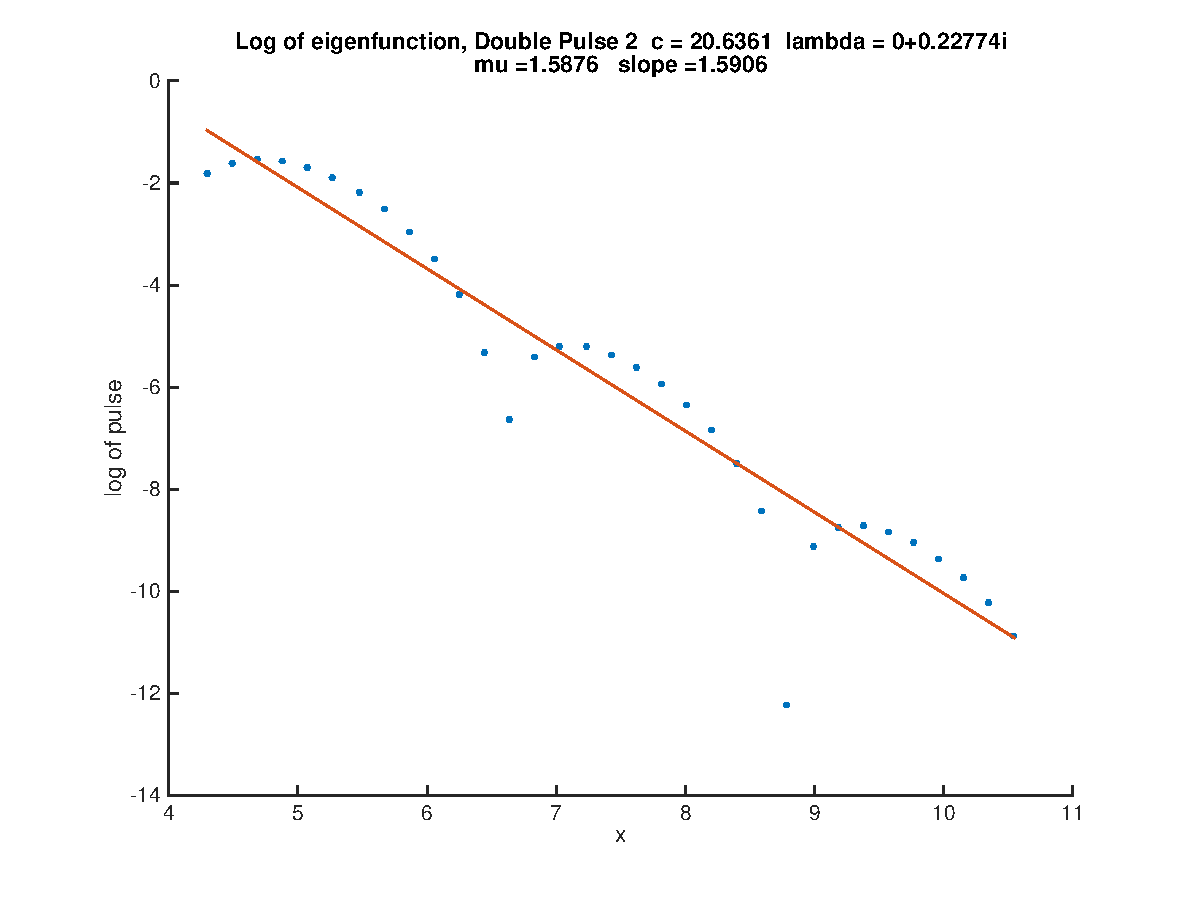
\includegraphics[width=8.5cm]{decay2.eps}
\end{figure}

\begin{figure}[H]
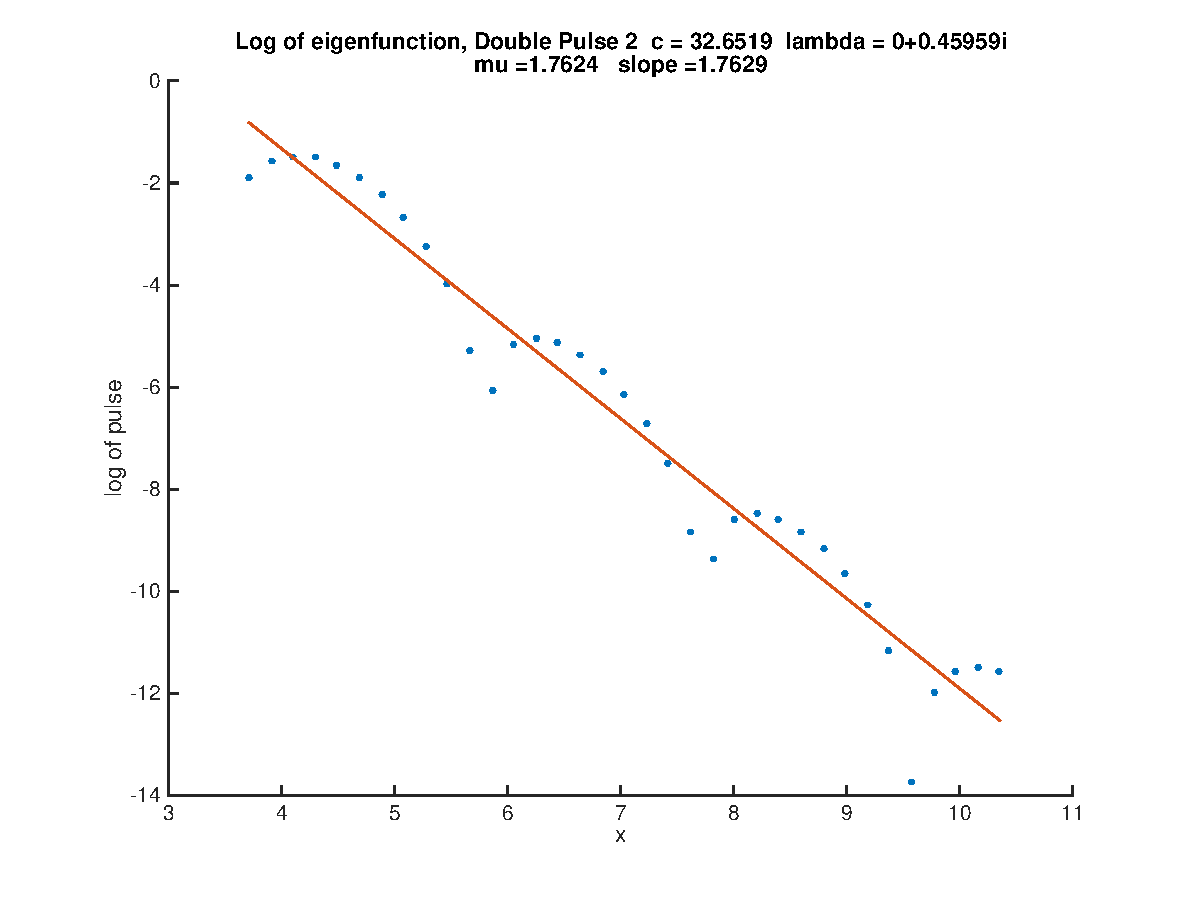
\includegraphics[width=8.5cm]{decay3.eps}
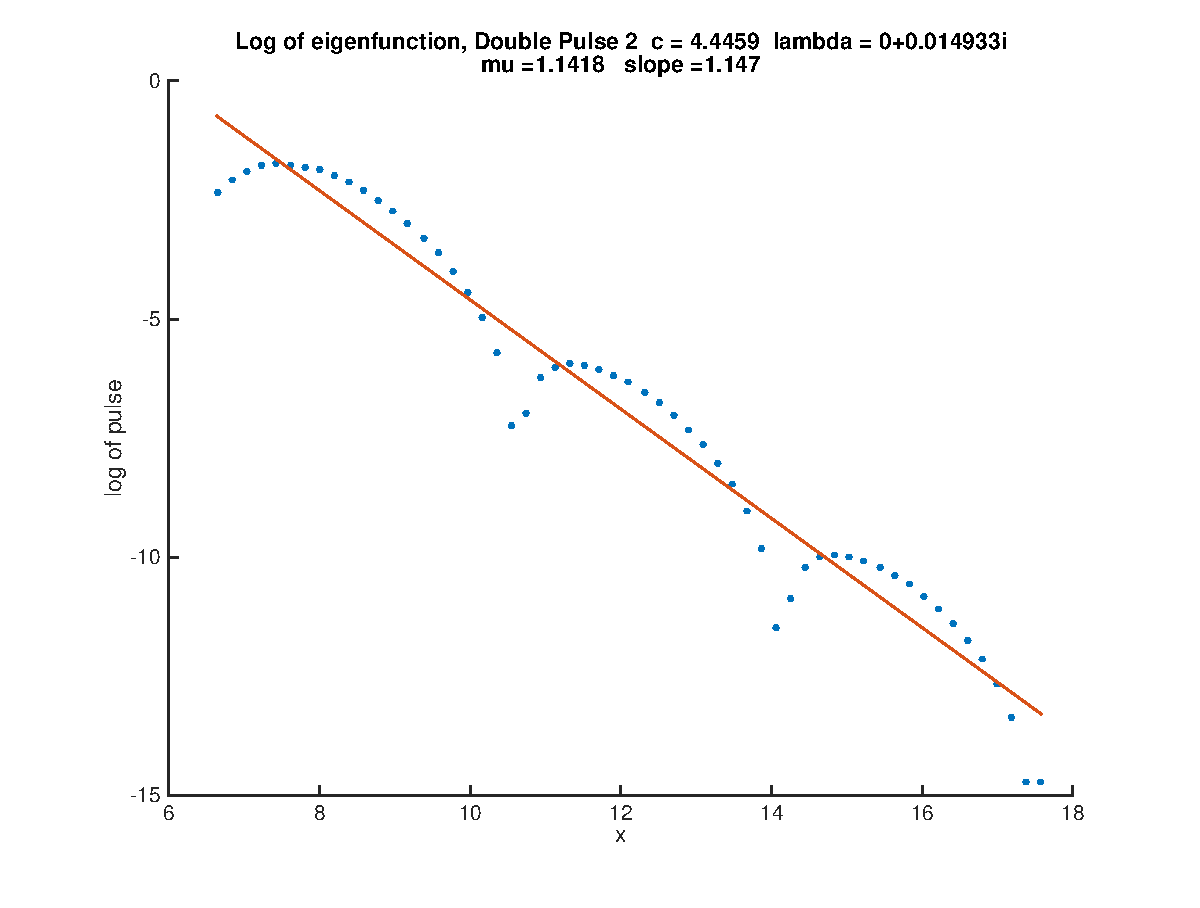
\includegraphics[width=8.5cm]{decay4.eps}
\end{figure}

The decay rate (slope of line) matches pretty well with the predicted decay rate ($\mu$). That being said, we are fitting a straight line to something with a linear trend but which is not linear due to the presence of oscillations. If we could figure out the approximate frequency of the oscillations, we might be able to get rid of them and then fit a better line. Not sure if this is necessary, though.


\subsection*{Symmetry of Solutions}
Recall that we previously discussed the symmetry (about the $y$-axis) of stationary solutions to our 5th order KdV equation (or the 4th order ODE we get after integrating the stationary problem once). We know that all such solutions (single pulse or multipulse) will be even functions. The solutions we were getting from Matlab's \texttt{fsolve} were not, because they had been translated by a tiny amount; since the equation is translation-invariant, these are still solutions, and \texttt{fsolve} has no way of picking out a unique one. Here we talk about ways to get a unique, centered solution out of \texttt{fsolve} by imposing an additional symmetry condition (phase condition). In all cases, we are looking to solve the (nonlinear) system $F(u) = 0$, where $F$ is the nonlinear 4th order differential operator.
\begin{enumerate}
  \item If $u_*(x)$ is a solution known to be even, and we are looking for a solution $u(x)$ which is ``close'' to that (e.g. the next step in a parameter continuation scheme), then we can use \texttt{fsolve} on the following system:
  \[ \begin{cases}
    F(u) = 0 \\
    \int u'(x)\left( u(x) - u_*(x)\right) dx = 0
  \end{cases} \]
  where the integral is taken over our domain ($[L, L]$ in the numerical schemes). The integral comes from minimizing the map;
  \[
  \tau \rightarrow \int \left( u(x+\tau) - u_*(x) \right)^2 dx
  \]
with respect to $\tau$. If $u_*(x)$ is even, this should yield an even function since the minimum should be at whatever value of $\tau$ we need to make $u(x+\tau)$ even. Although this does work, it requires incredibly small steps in the continuation code, so it is not very practical.
  \item We can also have \texttt{fsolve} minimize the (squared) L2 norm of $u(x) - u(-x)$, where $u(x)$ is the solution we are looking for. In other words, we can use \texttt{fsolve} on the following system:
  \[ \begin{cases}
    F(u) = 0 \\
    \int \left( u(x) - u(-x)\right)^2 dx = 0
  \end{cases} \]
  Since we are in the discrete world, we replace this with the discrete squared L2 norm. This method lets us use larger step sizes in the parameter continuation scheme as well as allows us to construct double pulses. Since the L2 norm of this difference is very small, we weight it more heavily by multiplying it by $1/\max(F(u))$, which makes it roughly the same order of magnitude as the other terms. \\

  Since this method works practically, we will use it. Here is a table comparing this method of symmetry enforcement to what we were doing before.

\begin{figure}[H]
\begin{tabular}{l|l|l|l|l}
Speed $c$    & Symmetry Enforcement & $\int(u(x) - u(-x))^2$ & $\max(F(u))$ & $\max |u(x) - u(-x)|$ \\ \hline
 0.64179 &  No   &  4.5045e-16 & 1.4988e-12  & 8.7368e-09 \\ 
         &  Yes  &  3.3368e-22 & 1.2754e-12  & 7.6337e-12 \\
  4.4934 &  No   &  1.0295e-12 &  1.706e-11  & 5.6763e-07 \\ 
         &  Yes  &  1.3277e-19 &  1.0232e-11 & 2.0375e-10 \\ 
\end{tabular}
\end{figure}
The symmetry-enforced solution is approximately as good a solution as the other version, and the degree of ``un-evenness'' is much smaller. We will use the same symmetry condition when constructing double pulses. It runs a little slower with this extra condition, but it is acceptable.

\end{enumerate}

\subsection*{Symmetry of Eigenfunctions, Theory}
Here we are interested in symmetry relations for eigenfunctions of the linearized 5th order problem about a stationary solution $u^*(x)$. Write the linearized 5th order problem about $u^*(x)$ as $Lv = \partial_x Hv = \lambda v$, where
\[
L = \partial_x( \partial_x^4 - \partial_x^2 + c - 2u^*)
\]


Suppose we have a solution to the eigenvalue problem, i.e.
\[
Lv(x) = \lambda v(x)
\]
i.e. $v(x)$ is an eigenfunction of linear operator $L$ corresponding to eigenvalue $\lambda$.
The following things are not hard to show:
\begin{enumerate}
	\item Since everything in the operator $L$ is real, $\bar{v}(x)$ is an eigenfunction of $L$ corresponding to eigenvalue $\bar{\lambda}$:
	\[
	L\bar{v}(x) = \bar{\lambda} \bar{v}(x)
	\]
	\item Now assume that the stationary solution $u^*(x)$ is an even function, i.e. $u^*(x) = u^*(-x)$. This is a reasonable assumption given what we know about this equation and that all stationary solutions we have found to it have been even functions. Then the derivative $\partial_x u^*(x)$ is an odd function, and we can show that $v(-x)$ is an eigenfunction of $L$ corresponding to eigenvalue $-\lambda$.
	\[
	Lv(-x) = -\lambda v(-x)
	\]
\end{enumerate}
Now suppose that our eigenvalue $\lambda$ is pure imaginary, i.e. $\lambda = i \beta$, where $\beta$ is real (and nonzero). Note that in this case, $\bar{\lambda} = -\lambda$, so let's see what that gets us. Write the eigenfunction as $v(x) = u(x) + i w(x)$, where $u(x)$ and $w(x)$ are both real. If we substitute these in, we get:
\[
L(u+iw) = i\beta(u+iw) = -\beta w + i u
\]
Using linearity and comparing real and imaginary parts, we get the pair of equations
\[ \begin{cases}
Lu = -\beta w \\
Lw = \beta u
\end{cases}\]
So the real and imaginary parts of $v(x)$ are related. If, say, we know the real part $u$, then the imaginary part $w$ is given by
\[
w = -\frac{1}{\beta}Lu
\]
Now let's use the fact that $\bar{\lambda} = -\lambda = -i \beta$ as well as the two facts we showed above. Writing down the eigenvalue problems for $\bar{v}(x) = u(x) - i w(x)$ and $v(-x) = u(-x) + i w(-x)$:
\begin{align*}
	L( u(x) - i w(x) ) &= i \beta ( u(x) - i w(x) ) \\
	L( u(-x) + i w(-x) ) &= i \beta ( u(-x) + i w(-x) )
\end{align*} 
So we have two distinct eigenfunctions corresponding to the same eigenvalue. Now assume that the eigenspace $E_\lambda$ is one-dimensional, i.e. the eigenvalue $\lambda$ is simple. I believe we know this is the case, but I'll look up the reference later. If that is true, than these two eigenfunctions are linearly dependent, so one must be a constant (nonzero) multiple of the other.
\begin{align*}
\bar{v}(x) &= k v(-x) \\
u(x) - i w(x) &= k( u(-x) + i w(-x) )
\end{align*}
where $k$ is complex. Write $k = re^{i\theta}$. First we show that $k$ must be a unit complex number, i.e. $r = 1$. There are many ways we can do this. One way is to look at the following three equations. The first is just our relation above, which is true for all $x$. For the second, we take $x \rightarrow -x$. For the third, we start with the second and take the complex conjugate of both sides.
\begin{align*}
\bar{v}(x) &= k v(-x) \\
\bar{v}(-x) &= k v(x) \\
v(-x) &= \bar{k} \bar{v}(x) 
\end{align*}
Substituting the third into the first, we get
\[
\bar{v}(x) = k \bar{k} \bar{v}(x) = |k|^2\bar{v}(x)
\]
for all $x$. Since $v$ is not the zero function, $\bar{v}(x)$ must be nonzero for at least one $x$, so we can cancel it from both sides to get $|k|^2 = 1$. Thus $k$ is a unit complex number, i.e. $k = e^{i\theta}$. Alternatively, we can multiply the two equations:
\begin{align*}
\bar{v}(x) &= k v(-x) \\
v(x) &= \bar{k} \bar{v}(-x)
\end{align*}
to get $|v(x)|^2 = |k|^2 |v(-x)|^2$. Integrating both sides over $\R$, since the eigenfunctions are in $L^2$ and the $L^2$ norms of $v(x)$ and $v(-x)$ are the same (and nonzero, since $v(x)$ is an eigenfunction), we get the same result. We are left with
\[
\bar{v}(x) = e^{i\theta}v(-x)
\]
Recall that both sides of this equation are eigenfunctions corresponding to eigenvalue $-i \beta$. Now multiply both sides by $e^{-i\theta/2}$. 
\[
e^{-i\theta/2}\bar{v}(x) = e^{i\theta/2}v(-x)
\]
Since we multiplied by a constant, both sides are still eigenfunctions corresponding to eigenvalue $-i \beta$. Let $v_*(x) = e^{i\theta/2} v(x)$. Since $\bar{v_*}(x) = e^{-i\theta/2} \bar{v}(x)$, our equation becomes
\[
\bar{v_*}(x) = v_*(-x)
\]
We finally have what we want, i.e. two identical eigenfunctions corresponding to eigenvalue $-i \beta$. Writing $v_*(x) = u_*(x) + i w_*(x)$, we get 
\[
 u_*(x) - i w_*(x) =  u_*(-x) + i w_*(-x)
\]
Finally, we equate real and imaginary parts to get
\[ \begin{cases}
u_*(-x) = u_*(x)&\text{real part $u_*(x)$ is even}\\
w_*(-x) = -w_*(x)&\text{imaginary part $w_*(x)$ is odd}
\end{cases}\]
We can write explicit formulas for $u_*(-x)$ and $w_*(-x)$ in terms of $u(-x)$ and $w(-x)$ and $\theta$.
\begin{align*}
v_*(x) &= e^{i\theta/2} v(x) \\
&= \cos(\theta/2) + i\sin(\theta/2)(u(x) + i w(x))\\
&= \left( u(x) \cos(\theta/2) - w(x) \sin(\theta/2) \right) + i \left( u(x) \sin(\theta/2) + w(x) \cos(\theta/2)\right)
\end{align*}
Comparing real and imaginary parts, we get
\begin{align*}
u_*(x) &= u(x) \cos(\theta/2) - w(x) \sin(\theta/2) \\
w_*(x) &= u(x) \sin(\theta/2) + w(x) \cos(\theta/2)
\end{align*}
Since $v_*(x) = e^{i\theta/2} v(x)$ is just multiplication of an eigenfunction by a constant (essentially a rotation), we have constructed an eigenfunction corresponding to $i \beta$ which has an even real part and an odd imaginary part. Can we show this numerically?

\subsection*{Symmetry of Eigenfunctions, Numerics}
We redo the numerics using our more-symmetric double pulses which we construct using the additional phase condition described above. Since the symmetry of the stationary solution $u^*(x)$ is essential to our argument above, it is important that our constructed double pulse be as symmetric as possible. We run the following experiement.
\begin{enumerate}
	\item Start with known solution at known value of $c$. Use Fourier spectral methods with $N = 256$, domain size $L = 25$.
	\item Run continuation code in parameter $c$ to achieve desired value of $c$. We will try several different ones.
	\item Construct Double Pulse 2 (first double pulse with pure imaginary eigenvalues).
	\item Find eigenfunction corresponding to positive imaginary eigenvalue.
	\item Look for the above symmetry in eigenfunction, or try to construct something better with the above symmetry.
\end{enumerate}

First we try this with (arbitrarily chosen) $c = 32.6519$. After constructing Double Pulse 2, we find (as expected) a pair of purely imaginary eigenvalues. The positive one is $\lambda = -9.7903e-12 + 0.4596i$. Note that we are using only 256 grid points here, and the real part of this is of order $1e-12$. Before we enforced symmetry, we got real parts of order $1e-5$. Already, the symmetry-enforcing version is looking better. Here are the real and imaginary parts of the corresponding eigenfunction $v(x)$.

\begin{figure}[H]
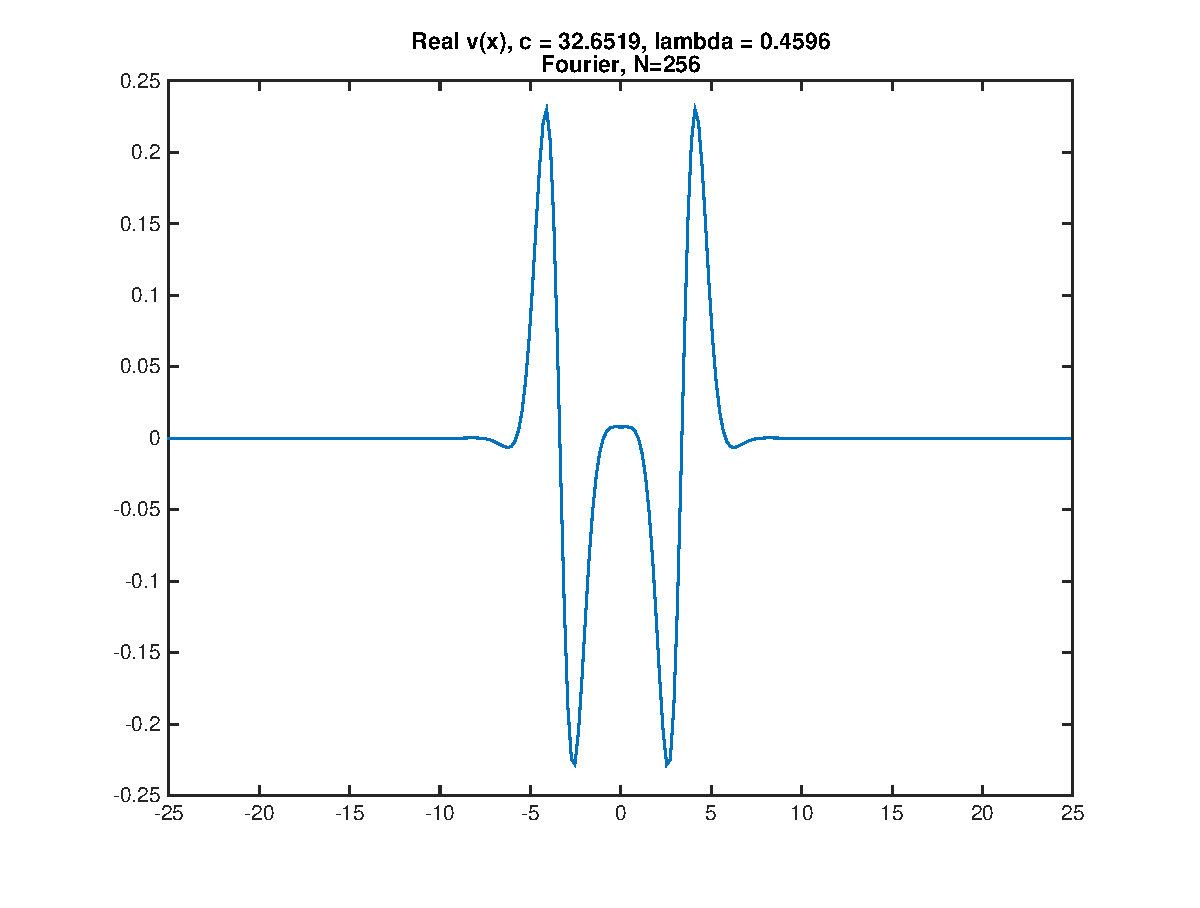
\includegraphics[width=8.5cm]{1eigenfnrealbefore.eps}
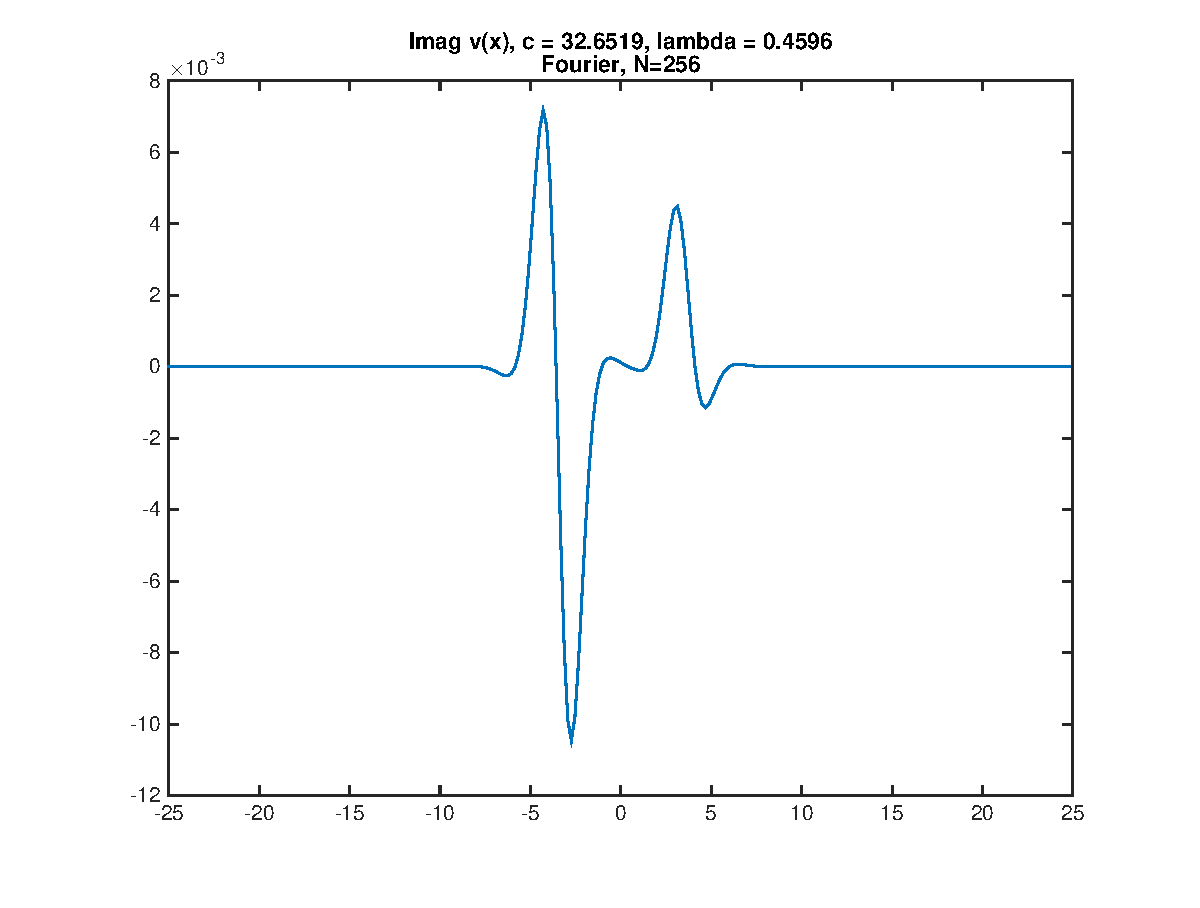
\includegraphics[width=8.5cm]{1eigenfnimagbefore.eps}
\end{figure}

The real part looks even when zoomed out, but when we zoom it, it is not quite symmetric, although it is very close ($\max |v(x) - v(-x)|$ is of order 1e-4). The imaginary part does not look like an odd function. Since this is not quite what we are looking for, we will try instead to construct what we want. Here is the procedure we will use. It's a little arbitrary, but it does give nice results.
\begin{enumerate}
	\item Start with real part $u(x)$, which we obtain from averaging together the real parts of $v(x)$ and $v(-x)$. This gives us an even function.
	\item Construct the imaginary part $w(x)$ by using the relation $w(x) = -\frac{1}{\beta}Lu(x)$; $\beta$is the imaginary part of the eigenvalue $\lambda$, which is 0.4596 in this case.
	\item Let $v(x) = u(x) + i w(x)$ be our candidate eigenfunction. Start \texttt{fsolve} at this function.
	\item Use \texttt{fsolve} with input $[u(x), w(x), \beta]$, i.e. allow the solver to adjust the real part of the eigenfunction, the imaginary part of the eigenfunction, or the imaginary part of the eigenvalue. The function whose zero we want is
	\[
	[ L u(x) + \beta w(x), L w(x) - \beta u(x) ]
	\]
	Note that: (1) we are forcing the eigenvalue to be pure imaginary, i.e. we are eliminating the small real part we found numerically; (2) this function is entirely real, so \texttt{fsolve} will only permit real output; (3) nowhere are we enforcing any symmetry (even or odd) for $u(x)$ or $w(x)$. The only symmetry we have is in the function we start with.
\end{enumerate}
Using this procedure, \texttt{fsolve} converges nicely, and we get the following results:
\begin{figure}[H]
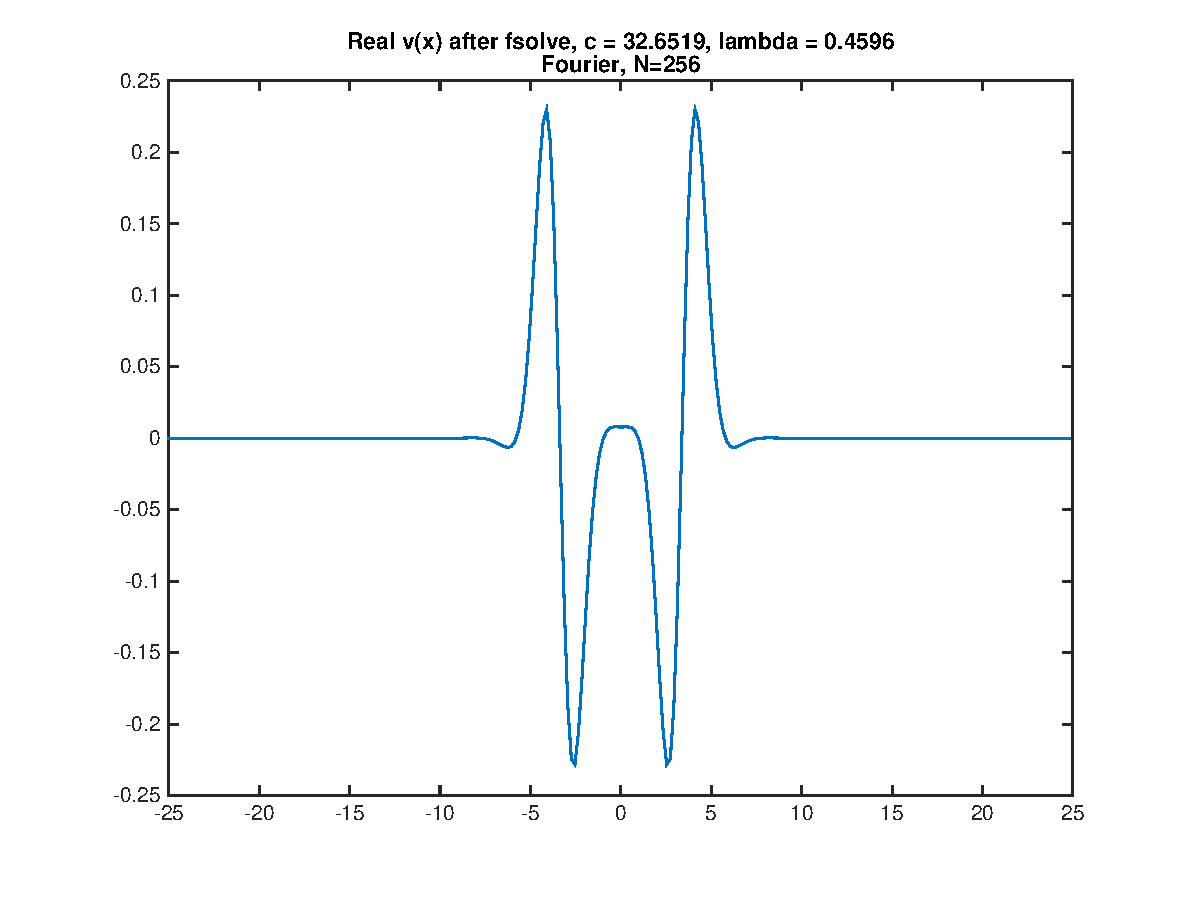
\includegraphics[width=8.5cm]{1eigenfnrealafter.eps}
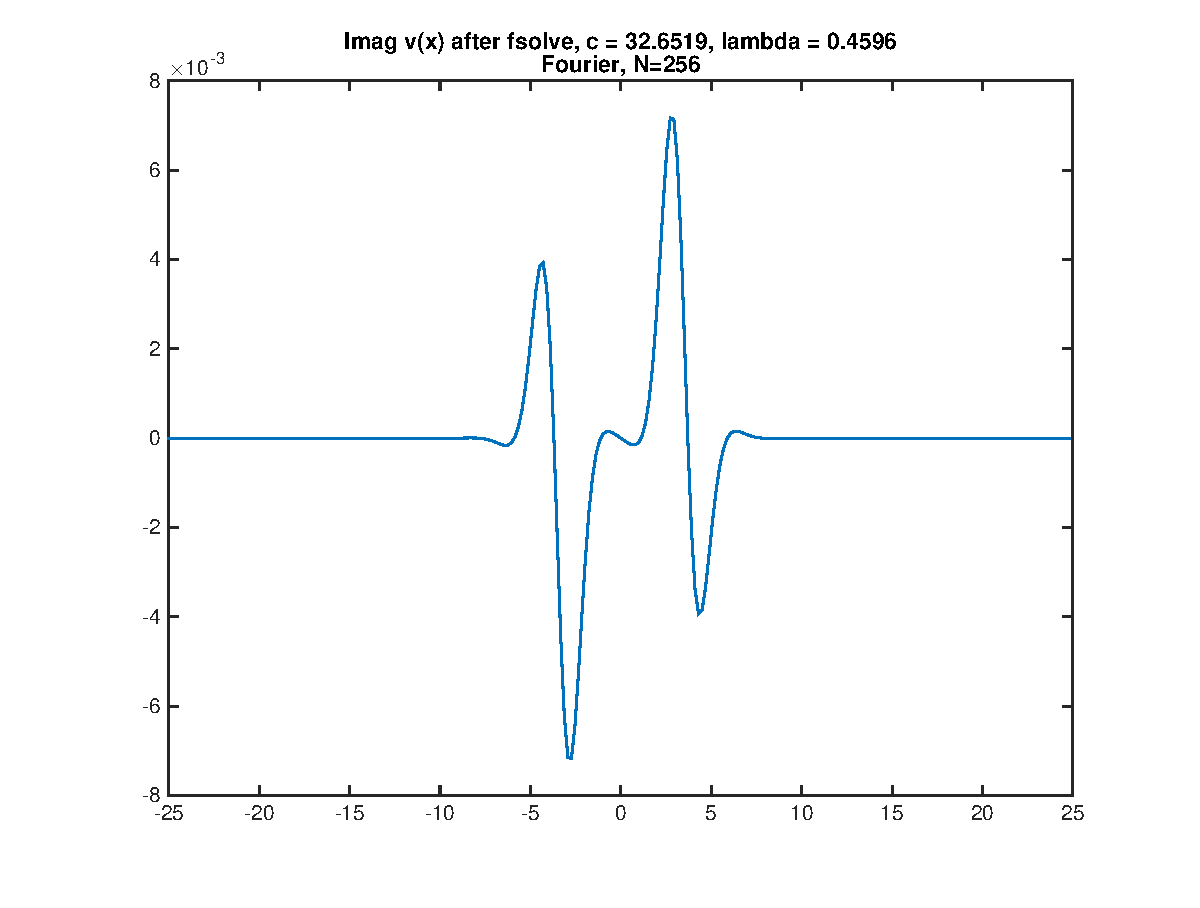
\includegraphics[width=8.5cm]{1eigenfnimagafter.eps}
\end{figure}
The real part looks even, and is much more even when we zoom in. The imaginary part now looks like a nice odd function. Interestingly, the imaginary part of the eigenvalue has shifted by $5.1331e-10$, which we allowed for in our procedure. Since the plots look good, let's do some quantitative comparison. In all that follows, $v(x)$ is the eigenfunction with eigenvalue $\lambda = i \beta$, $u(x)$ is the real part of $v(x)$, and $w(x)$ is the imaginary part of $v(x)$.

\begin{figure}[H]
\begin{tabular}{l|l|l}
 Double Pulse 2, $c = 32.6519, \lambda=0.4596i$  & Before \texttt{fsolve} & After \texttt{fsolve} \\ \hline
$\max|Lv(x) - \lambda v(x)|$  & 3.6193e-11 & 6.8845e-12 \\ 
$\max|u(x) - u(-x) |$         & 2.1030e-04 & 3.0855e-10 \\
$\max|w(x) + w(-x) |$         &  0.0067    & 9.6587e-12 \\
$\max|w(x) + (1/\beta)Lu(x)|$ &  8.0953e-11& 2.0272e-11 \\
\end{tabular}
\end{figure}
This looks good. By all measures, the post-\texttt{fsolve} solution is better. In addition, its real part is even and its imaginary part is odd to order $1e-10$ numerically. Thus we have verified our theoretical result numerically. Just to be safe, we should try this for another value of $c$. How about something much smaller? The plots (not shown) look similar to those above, so here is the quantitative comparison.

\begin{figure}[H]
\begin{tabular}{l|l|l}
 Double Pulse 2, $c = 4.4459, \lambda=0.0149i$  & Before \texttt{fsolve} & After \texttt{fsolve} \\ \hline
$\max|Lv(x) - \lambda v(x)|$  & 5.5157e-11 & 6.5550e-12 \\ 
$\max|u(x) - u(-x) |$         & 6.7461e-05 & 1.3578e-13 \\
$\max|w(x) + w(-x) |$         & 0.0047     & 4.3774e-12\\
$\max|w(x) + (1/\beta)Lu(x)|$  & 3.7036e-09 & 2.0272e-11 \\
\end{tabular}
\end{figure}
Again, everything looks better after \texttt{fsolve}. Let's do one more value of $c$, and this time we will look at Double Pulse 2 and Double Pulse 4. The plots (not shown) look good, so here are the numbers.

\begin{figure}[H]
\begin{tabular}{l|l|l}
 Double Pulse 2, $c = 9.4812, \lambda=0.0629i$  & Before \texttt{fsolve} & After \texttt{fsolve} \\ \hline
$\max|Lv(x) - \lambda v(x)|$  & 5.7609e-11 & 5.3622e-12 \\ 
$\max|u(x) - u(-x) |$         & 8.8770e-05 & 2.3131e-13 \\
$\max|w(x) + w(-x) |$         & 0.0041     & 1.5354e-11 \\
$\max|w(x) + (1/\beta)Lu(x)|$ & 9.4213e-10 & 1.2168e-10 \\
$|\int v(x) dx|$              & 2.8938e-07 & 2.8937e-07 \\
\end{tabular}
\end{figure}

\begin{figure}[H]
\begin{tabular}{l|l|l}
 Double Pulse 4, $c = 9.4812, \lambda=0.0015i$  & Before \texttt{fsolve} & After \texttt{fsolve} \\ \hline
$\max|Lv(x) - \lambda v(x)|$  & 3.3100e-11 & 9.4437e-12 \\ 
$\max|u(x) - u(-x) |$         & 8.8770e-05 & 1.2434e-11 \\
$\max|w(x) + w(-x) |$         & 2.4242e-04 & 2.0247e-10 \\
$\max|w(x) + (1/\beta)Lu(x)|$ & 2.1726e-05 & 7.2353e-09 \\
$|\int v(x) dx|$              & 2.9558e-09 & 2.5906e-09 \\
\end{tabular}
\end{figure}

Once again, this looks good. Conclusion: the theoretical results are verified numerically. For the eigenfunction corresponding to a purely imaginary eigenvalue, we can construct an eigenfunction with a nice symmetry relationship: the real part is an even function and the imaginary part is an odd function. For this example, we also included the absolute value of the integral of the eigenfunction (should be 0). This was essentially unaffected by \texttt{fsolve} and has about the same order of magnitude it did before. If we like, we can also increase the number of grid points, but this is really slow. (The split real/imaginary \texttt{fsolve}) is the bottleneck; we could probably make it faster by using its Jacobian, but I don't think we need to). In any case, we get the same results with more grid points.\\

After revising the theoretical section above, I came up with another way of constructing an eigenfunction with desired symmetry. Let $v(x)$ be the eigenfunction produced by \texttt{eig}. Then we can use \texttt{fsolve} to find $\theta$ such that the real part of $v_*(x) = e^{-i \theta/2} v(x)$ is an even function, i.e. the discrete $L^2$ norm of $v_*(x) - v*(-x)$ is as close to 0 as possible. Let's try this for Double Pulse 2, $c = 9.4812$. Here are the real and imaginary parts of the eigenfunction corresponding to $\lambda = 0.0629i$ which are produced by \texttt{eig}.

\begin{figure}[H]
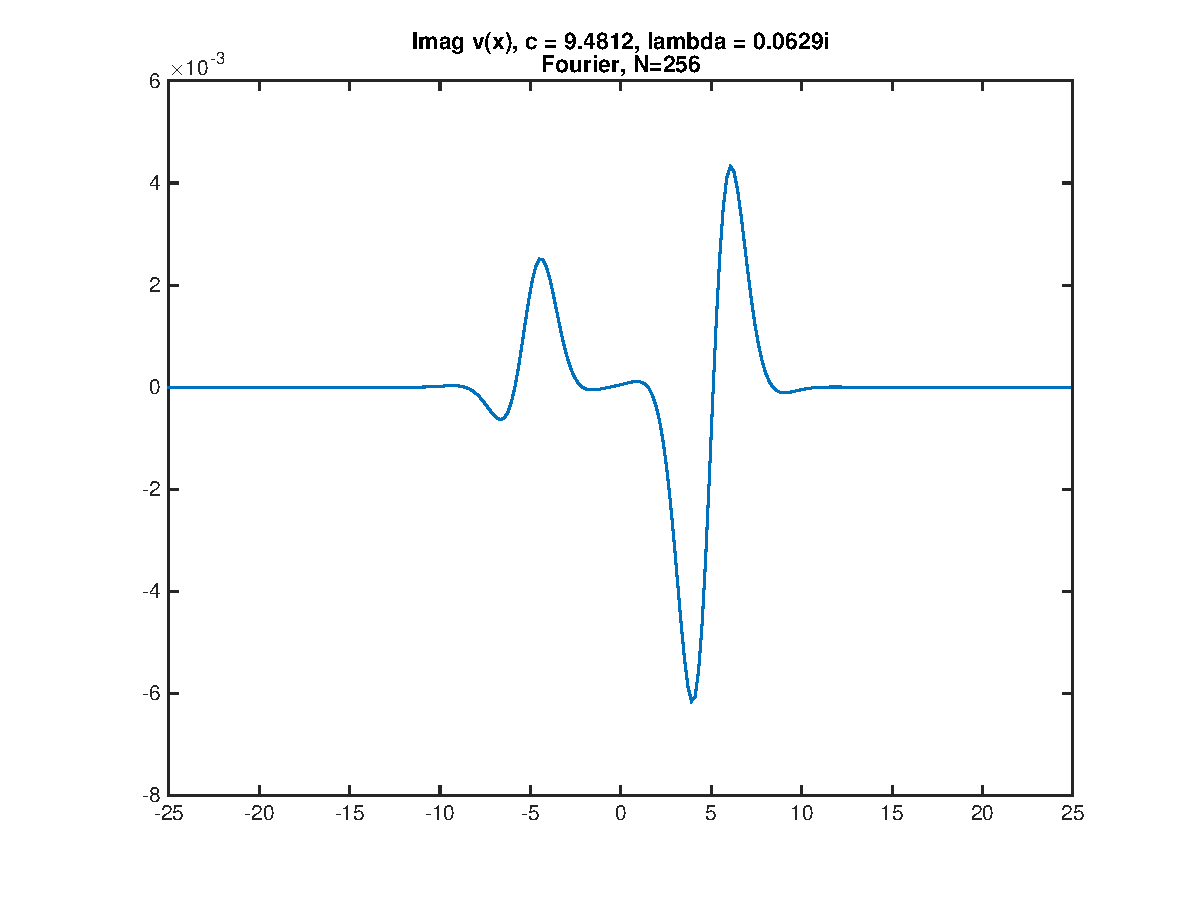
\includegraphics[width=8.5cm]{2eigenfnreal.eps}
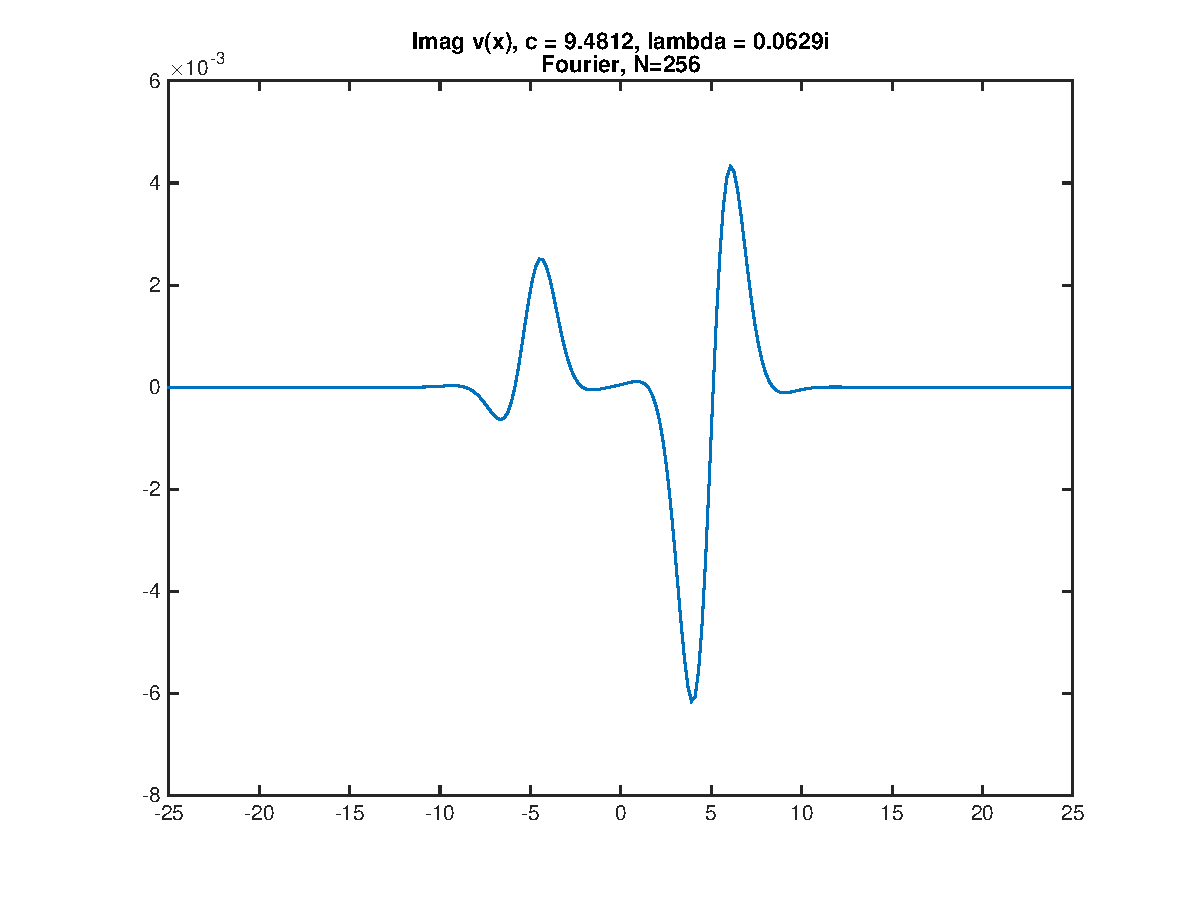
\includegraphics[width=8.5cm]{2eigenfnimag.eps}
\end{figure}

Here are the real and imaginary parts of the eigenfunction corresponding to $\lambda = 0.0629i$ after we use \texttt{fsolve} to rotate them by an angle $\theta$ so that the real part is an even function.

\begin{figure}[H]
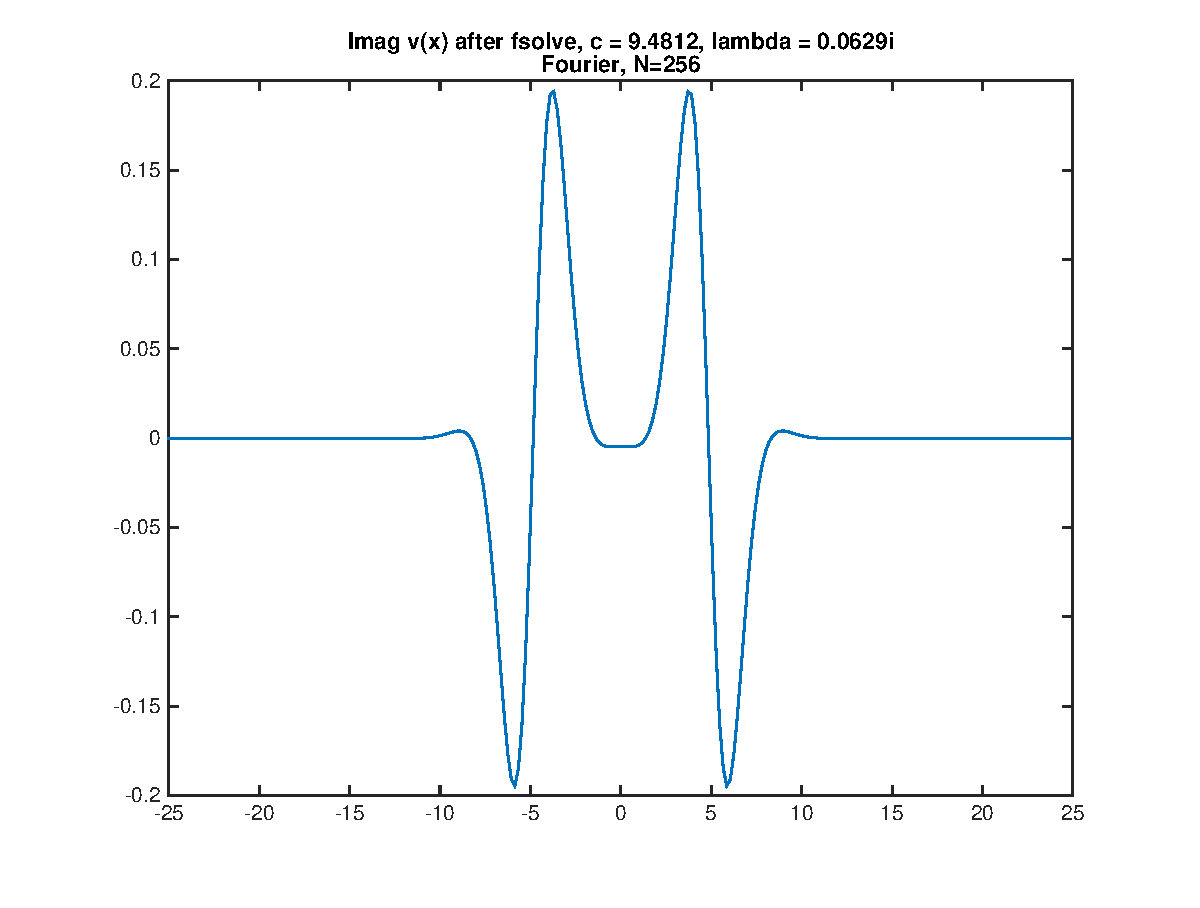
\includegraphics[width=8.5cm]{2eigenfnrealafter.eps}
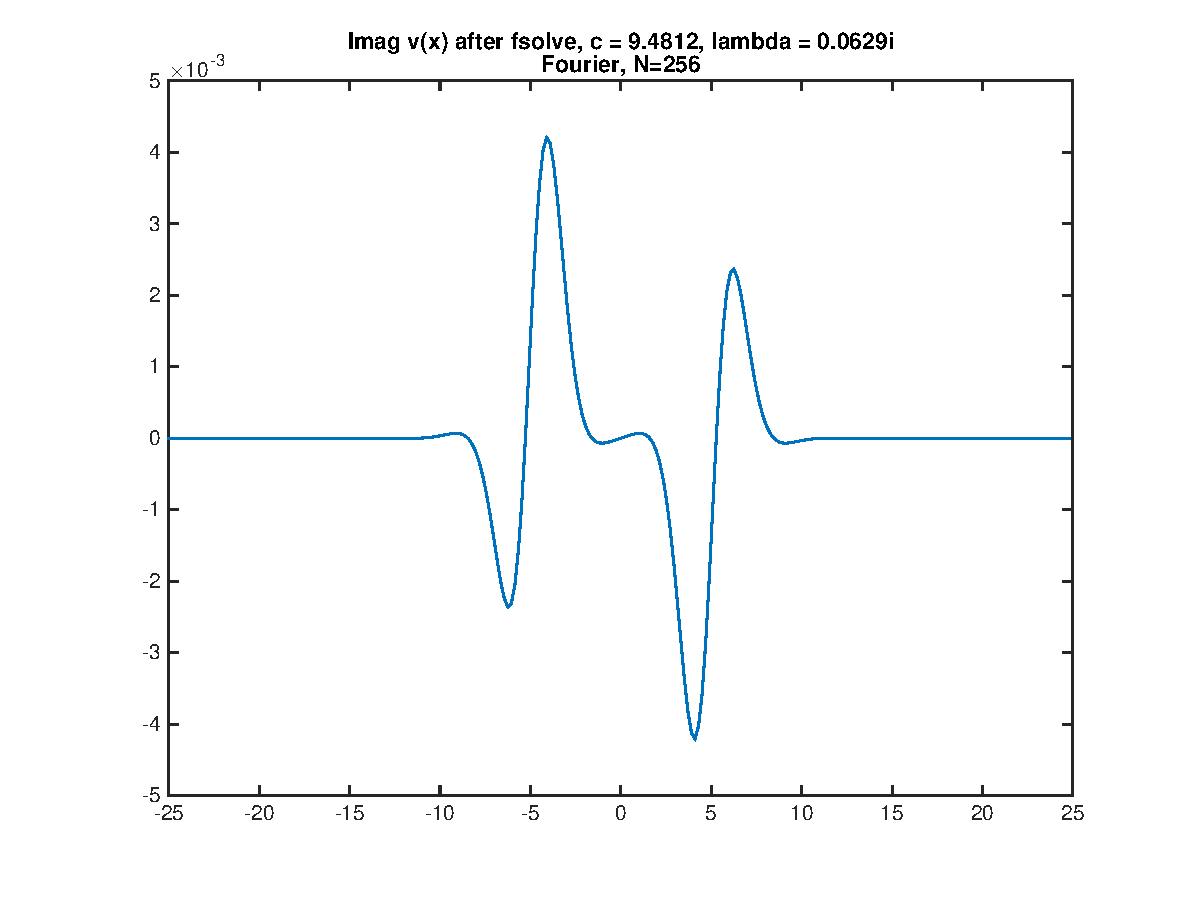
\includegraphics[width=8.5cm]{2eigenfnimagafter.eps}
\end{figure}

These certainly look much better. Let's look at the numbers. After we do the rotation, we do a second \texttt{fsolve} to remove the small real part of the eigenvalue.

\begin{figure}[H]
\begin{tabular}{l|l|l|l}
 Dbl P, $c = 9.4812, \lambda=0.0629i$  & Output from \texttt{eig} & After Rotation \texttt{fsolve} & After Second \texttt{fsolve}\\\hline
$\max|Lv(x) - \lambda v(x)|$  & 5.7609e-11 & 5.8482e-11 & 5.9202e-12 \\ 
$\max|u(x) - u(-x) |$         & 8.8770e-05 & 3.2920e-09 & 3.2727e-09 \\
$\max|w(x) + w(-x) |$         & 0.0041     & 1.3023e-07 & 1.3021e-07 \\
$|\int v(x) dx|$              & 2.8938e-07 & 2.8938e-07 & 2.8938e-07 \\
\end{tabular}
\end{figure}

Although the symmetry is not quite as good as when we enforced it manually above by averaging, these results are pretty good and are consistent with our theory. 

\end{document}

